\chapter{VRゲーム上で振動刺激のある魔法体験における没入感体験向上システム}
本研究では、VRを用いてユーザーの魔法体験における没入感を向上させるシステムを提案、開発し、視覚エフェクトと振動刺激の組み合わせによってユーザーの没入感にどのような影響を与えるのかを調査する.


\begin{figure}[b]
\centering
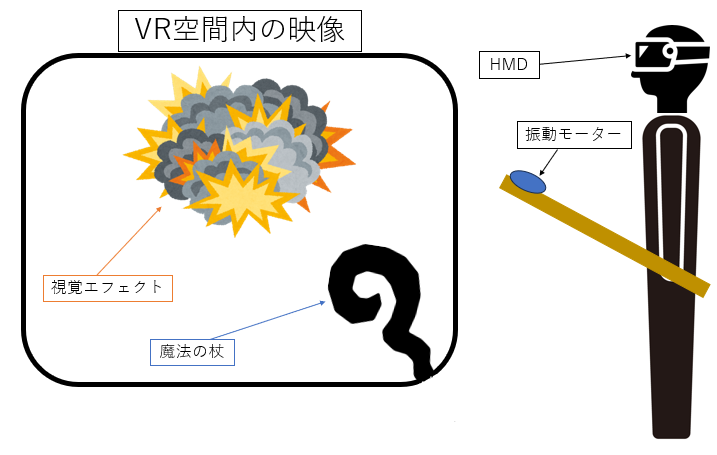
\includegraphics[clip,width=8cm]{./fig/allsystem.png}
\caption{システム概要}\label{allsystem}
\end{figure}

%%%%%%%%%%%%%%%%%%%%%%%%%%%%%%%%%%%%%%%%%%%%%%%%%%%%%%%%%%%%%%%%%%%%%%%
\begin{comment}
    \begin{textblock}{4.5}(1, 21.5)
        \noindent
        【16,18】表番号は章ごとの通し番号で抜けがない
    \end{textblock}
    \begin{textblock}{5}(14.5, 13)
        ←表のキャプションは上
    \end{textblock}
\end{comment}
%%%%%%%%%%%%%%%%%%%%%%%%%%%%%%%%%%%%%%%%%%%%%%%%%%%%%%%%%%%%%%%%%%%%%%%
\section{システム概要}
\figref{allsystem}に本システムの概要を示す.

本研究ではユーザーがヘッドマウントディスプレイを装着した上で,視覚エフェクトと振動刺激を体験してもらう.
視覚エフェクトと振動パターンは実験者が変更する.


視覚エフェクトのパターンは\figref{fire}\figref{explosion}\figref{ringfire}に示す.
と振動刺激のパターンは\figref{patarn1}\figref{patarn2}\figref{patarn3}に示す.



\section{魔法の形状と振動パターンの選定}
実装する視覚エフェクトは、形状が異なりユーザーに与えられる振動刺激が異なるであろう3種類の視覚エフェクトを選定した.
以下に選定した3種類の視覚エフェクトを示す.
\begin{figure}[h]
\centering
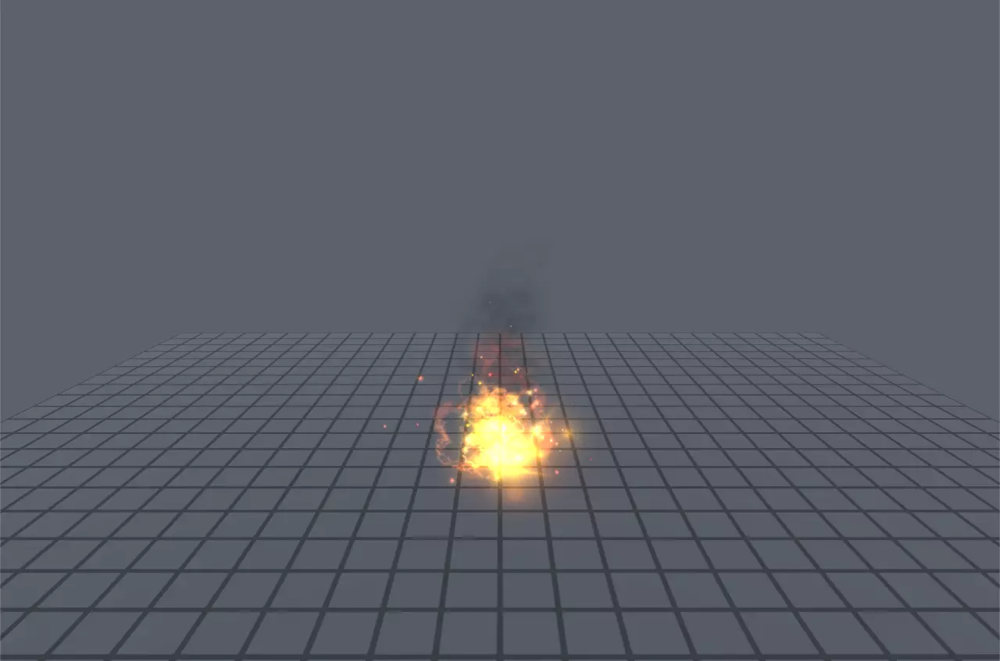
\includegraphics[clip,width=8cm]{./fig/firefire.png}
\caption{火}\label{fire}
\end{figure}

\begin{figure}[h]
\centering
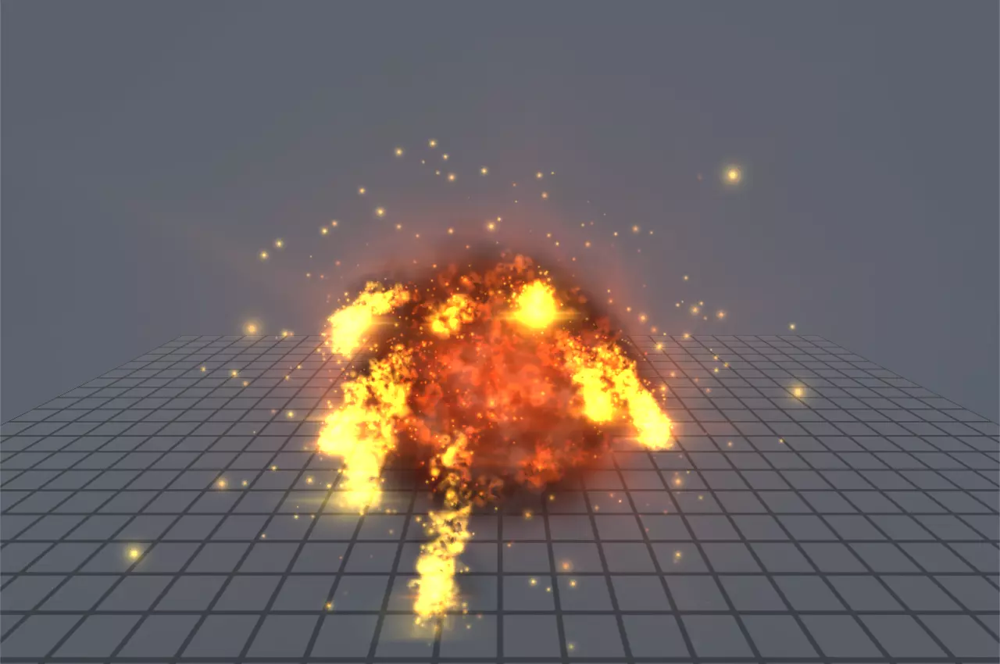
\includegraphics[clip,width=8cm]{./fig/explosion.png}
\caption{爆発}\label{explosion}
\end{figure}

\begin{figure}[h]
\centering
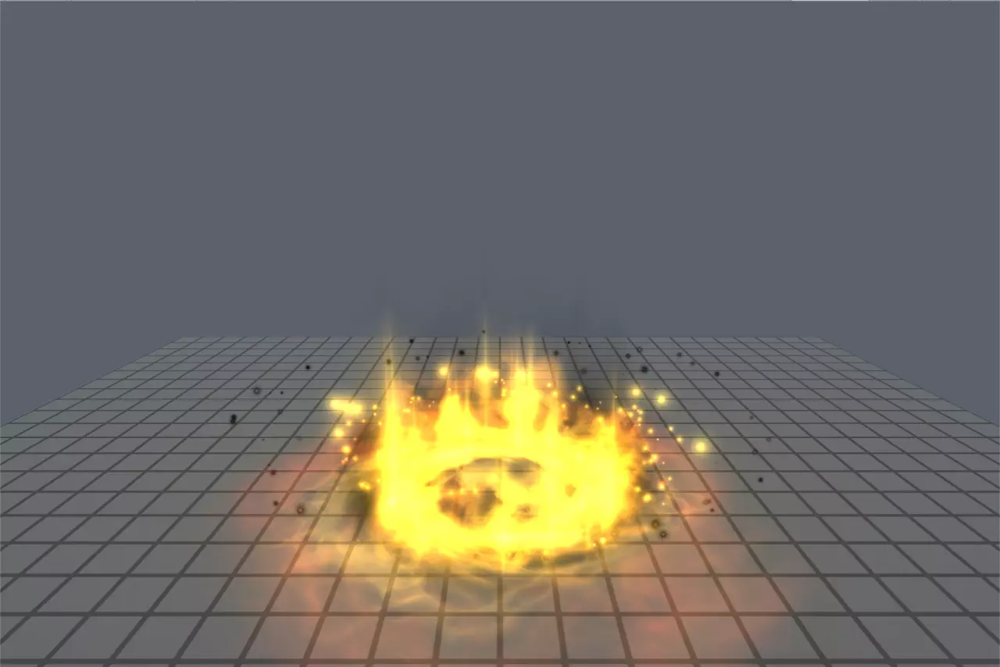
\includegraphics[clip,width=8cm]{./fig/ringfire.png}
\caption{円焔}\label{ringfire}
\end{figure}


振動パターンについては、



\begin{figure}[b]
\centering
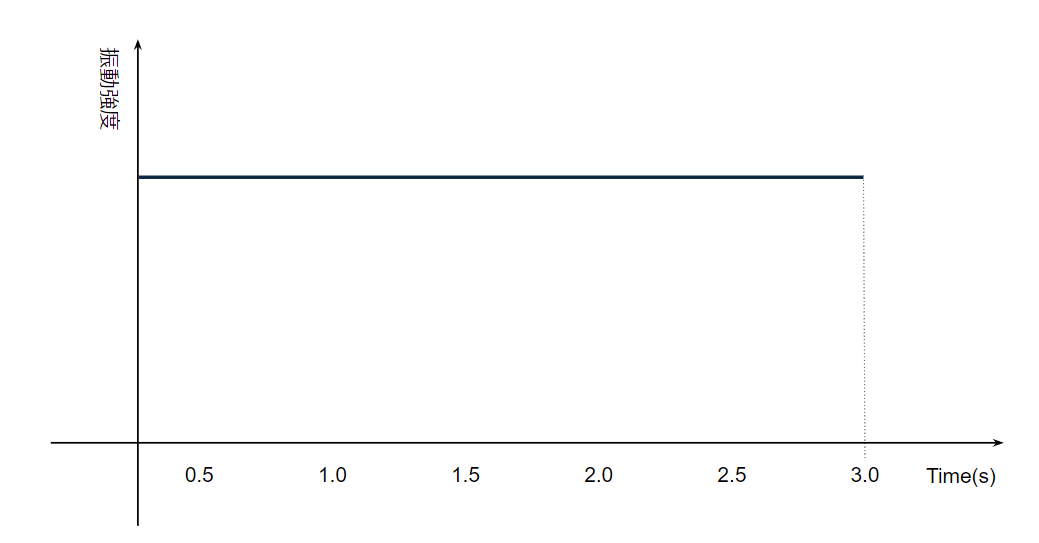
\includegraphics[clip,width=8cm]{./fig/patarn1.png}
\caption{パターン1}\label{patarn1}
\end{figure}

\begin{figure}[b]
\centering
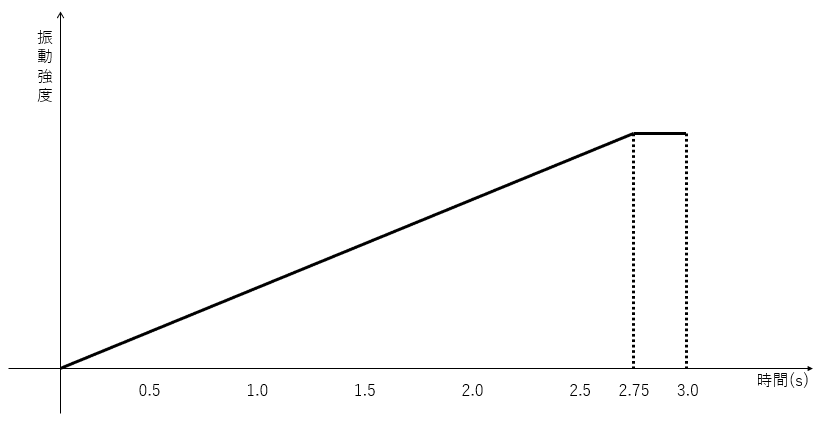
\includegraphics[clip,width=8cm]{./fig/patarn2.png}
\caption{パターン2}\label{patarn2}
\end{figure}

\begin{figure}[b]
\centering
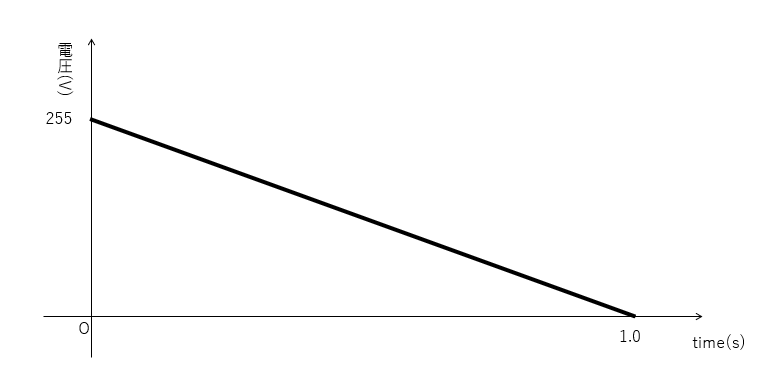
\includegraphics[clip,width=8cm]{./fig/patarn3.png}
\caption{パターン3}\label{patarn3}
\end{figure}

